\usetikzlibrary{arrows}
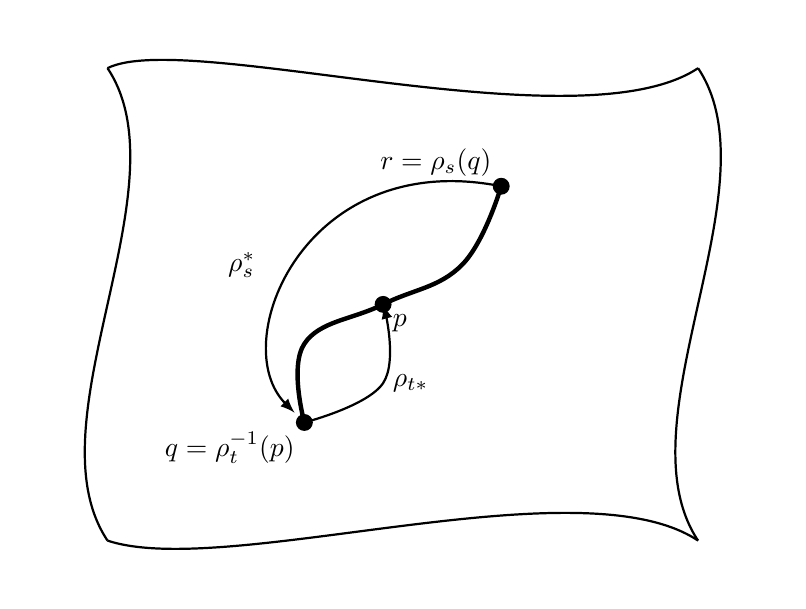
\begin{tikzpicture}



\node at (1,1) {};


\draw [thick] (-6,-4) .. controls (-7,-2.5) and (-5,0.5) .. (-6,2);
\draw [thick] (-6,2) .. controls (-5,2.5) and (0,1) .. (1.5,2);
\draw [thick] (1.5,2) .. controls (2.5,0.5) and (0.5,-2.5) .. (1.5,-4);
\draw [thick] (1.5,-4) .. controls (0,-3) and (-4.5,-4.5) .. (-6,-4);

\node [below left] (p) at (-3.5,-2.5) {$q = \rho_t^{-1}(p)$};
\node [below right] (q) at (-2.5,-1) {$p$};
\node [above left] (r) at (-1,0.5) {$r = \rho_s(q)$};

\node (p') at (-3.5,-2.5) {};
\node (q') at (-2.5,-1) {};
\node (r') at (-1,0.5) {};

\draw [fill = black] (p') circle (0.1);
\draw [fill = black] (q') circle (0.1);
\draw [fill = black] (r') circle (0.1);

\draw [ultra thick]  plot[smooth, tension=.7] coordinates {(p') (-3.5,-1.5) (q') (-1.5,-0.5) (r')};

\draw [thick, -latex] plot[smooth, tension=.7] coordinates { (p') (-2.5,-2) (q') };
\draw [thick, -latex](-1,0.5) .. controls (-3.5,1) and (-4.5,-1.5) .. (p');

\node [left] at (-4,-0.5) {$\rho_s^*$};
\node [right] at (-2.5,-2) {$\rho_{t*}$};

\end{tikzpicture}